%!TEX root = ./main.tex

%-------------------------------------
%-------------------------------------
% The model
%-------------------------------------
%-------------------------------------
\section{The model}

%\subsection{The model}

\begin{frame}{Our model}

\alert{Goal}: given a set of $n$ data with $p$ variables, infer the block structure of their variables
without knowing the number of groups.

\pause

\alert{Additional constraints}: 
\begin{itemize}
    \item use a Stochastic Block Model    
    \item the partition must respect the original order of the variables
\end{itemize} 

\pause

\alert{The model}: 
\begin{align*}
    \bm{y}_1, \ldots, \bm{y}_n \mid \bm{K} & \iid \mathcal{N}_p(\mathbf{0}, \bm{K}^{-1} ) \\
    \bm{K} \mid G & \sim \GWish(b, D)\\
    P((i,j)&\in E\mid \bm{z},Q) = Q_{z_{i} z_{j}},\,\text{independent}\\
        Q_{rs} \mid \bm{z} &\ind \Beta(a,b), 1\leq r\leq s\leq H\\
    \rho_p & \sim \mathcal{L}\left(\rho_p\right)
\end{align*}

% TODO inserire la prior?

\end{frame}


%-------------------------------------
%-------------------------------------
% The sampling strategy
%-------------------------------------
%-------------------------------------
\section{Sampling strategy}

\subsection{Overview of the sampling strategy}
\begin{frame}{Gibbs sampler}

formula del Gibbs sampler



\end{frame}




%-------------------------------------
% BDgraf
%-------------------------------------
\subsection{Updating the graph}
\begin{frame}{Birth and death algorithm for updating the graph}

   slide su bdgraph

\end{frame}


%-------------------------------------
% Updating the current partition
%-------------------------------------
\subsection{Updating the partition}


\begin{frame}{General steps for updating the partition}
    
    We perform an (adaptive) \alert{split and merge} as in \cite{bensonAdaptiveMCMCMultiple2018}.
    \begin{enumerate}
        \item With probability $\alpha_{\text{split}}$, usually $0.5$, choose an \alert{split move (add)}, otherwise a \alert{merge move (delete)}.
        \begin{enumerate}
            \item Propose a new partition by splitting one group into two or merging two adjacent ones.
            \item Accept or reject using Metropolis Hastings. The target is:
            $f(\rho \mid G) \approx f_G(G \mid \rho) f_{\rho}(\rho)$
            \[
                \alpha_{\text{accept,merge}} = \min % TODO non sono sicuro che qua ci vada del/merge, nelle note non aggiornate c'era add
                \bigg\{1,
                \underbrace{\frac{f_G\left(G \mid \rho'\right)}{f_G(G \mid \rho)}}_{\substack{\text{likelihood}\\\text{ratio}}}
                \underbrace{\frac{f_\rho\left(\rho'\right)}{f_\rho(\rho)}}_{\substack{\text{prior}\\\text{ratio}}}
                \underbrace{\frac{P(\text{choose merge})}{P(\text{choose split})} \frac{P(\text{merge})}{P(\text{split})}}_{\text{proposal ratio}}
                \bigg\}
            \]
        \end{enumerate}
        \item To improve the mixing of the chain we also perform a \alert{shuffle move}.
        \begin{enumerate}
            \item Propose a new partition by moving some nodes from a group to an adjacent one.
            \item Accept it using Metropolis Hastings
        \end{enumerate}

    \end{enumerate}

\end{frame}




\begin{frame}{Proposal ratio}

   slide su proposal ratio

\end{frame}




\begin{frame}{Adaptive step}

   non ho ben capito , vuole solo una slide sulla parte adattiva?
   forse è un po' troppo breve per una slide sola

\end{frame}



%-------------------------------------
%-------------------------------------
% Next steps
%-------------------------------------
%-------------------------------------
\section{Next steps}
\begin{frame}{Next steps}

    \begin{itemize}
        \item Praying that the code works
    \end{itemize}



\end{frame}



%----------------------------------------
% References
%-------------------------------------

\begin{frame}{Main references}
    % GGM
    \nocite{colombiLearningBlockStructured2022a}
    \nocite{mohammadiBayesianStructureLearning2015a}
    % SBM
    \nocite{legramantiExtendedStochasticBlock2022}
    % Changepoint
    \nocite{bensonAdaptiveMCMCMultiple2018}
    \nocite{martinezNonparametricChangePoint2014}
    
    
    %biblatex
    \printbibliography
    \renewcommand*{\bibfont}{\small}
    %bibtex
    %\bibliographystyle{plain} % We choose the "plain" reference style
    %\bibliography{bibliography} % Entries are in the refs.bib file
\end{frame}



\begin{frame}[plain]
    % Add background to content page
    \AddToShipoutPictureFG*{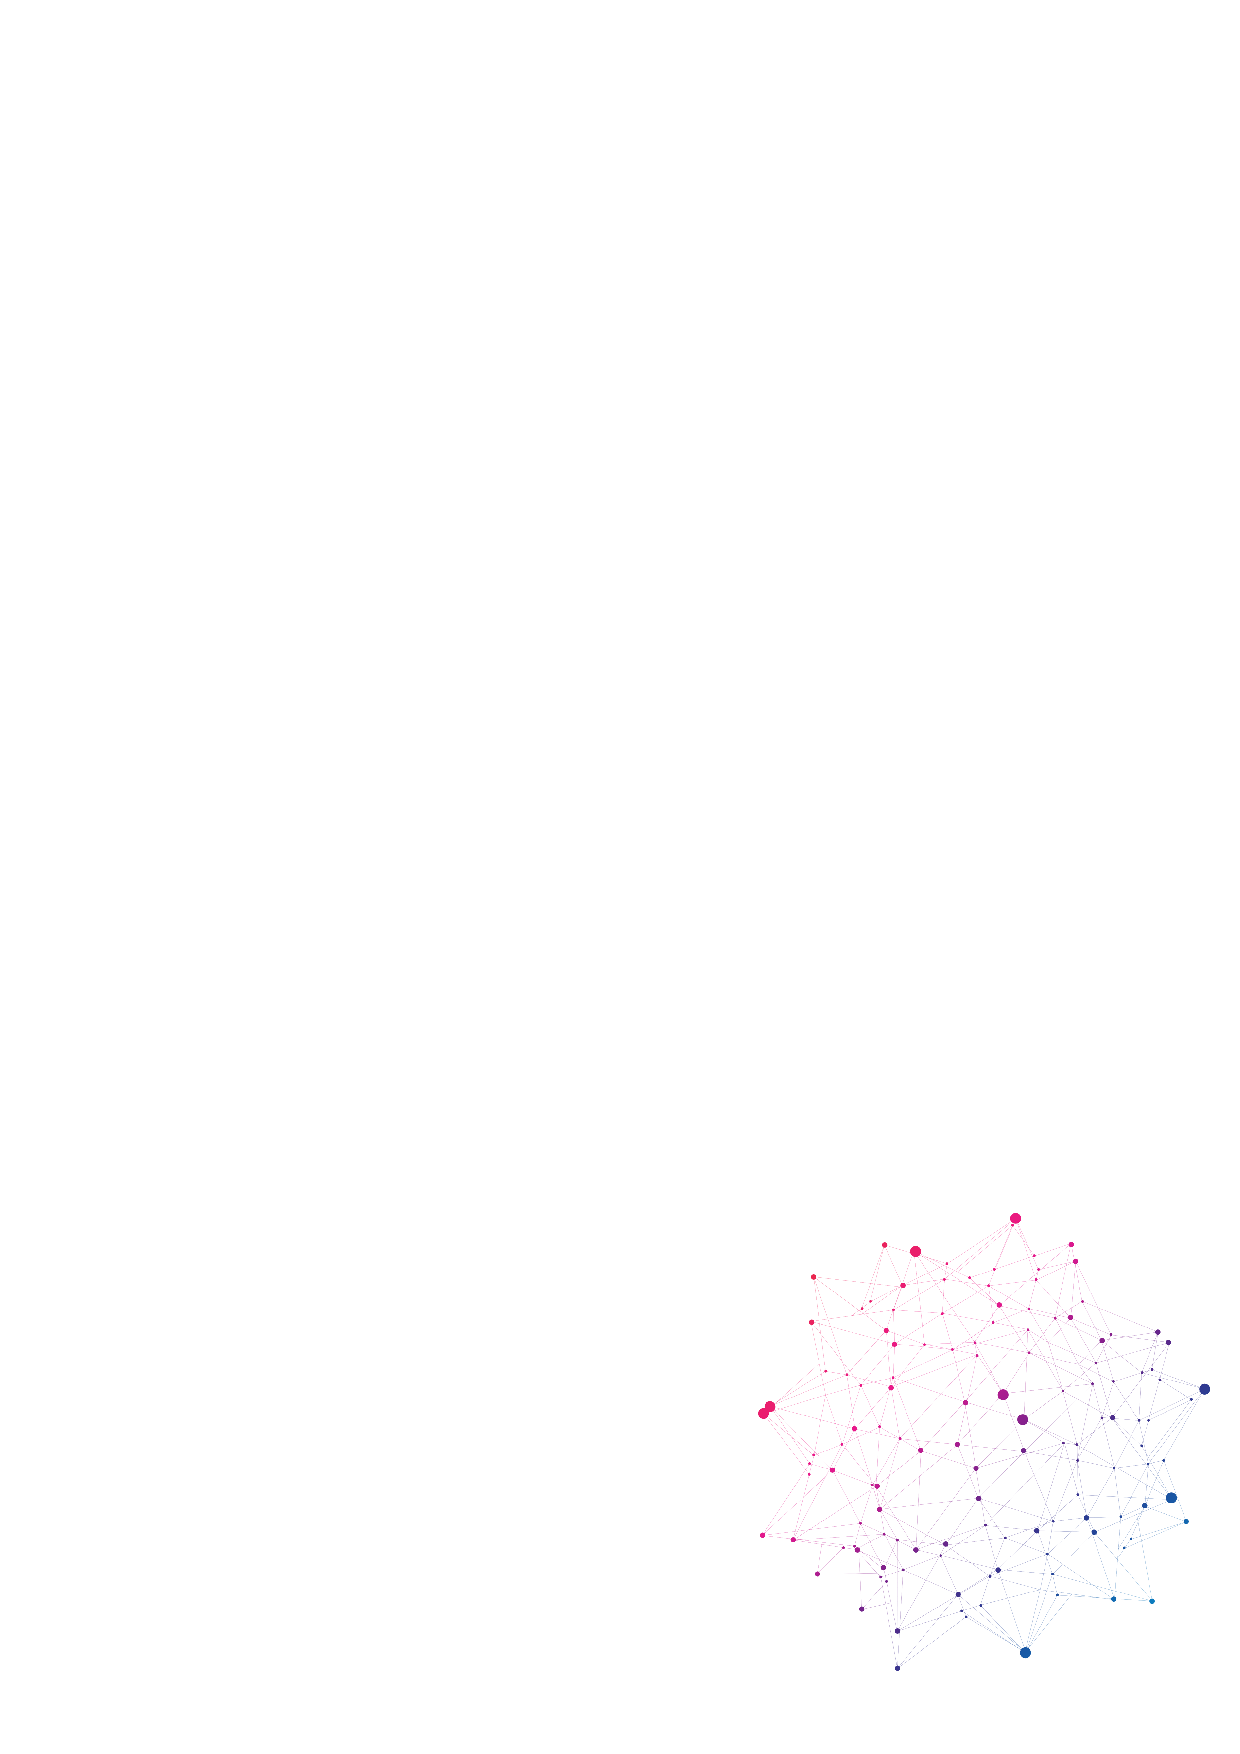
\includegraphics[width=\paperwidth]{Images/background.pdf}}
    \vspace*{1.2cm}
    \hspace*{1cm}{\Large Thank you!}\\
    \vspace*{0.6cm}
    \hspace*{1cm}{\Huge \alert{Any questions?}}
\end{frame}





%tenere?
\section*{Extra}

\begin{frame}{Extra content}


\end{frame}


